\documentclass[11pt,a4paper]{article}

\usepackage[margin=2.5cm]{geometry}
\usepackage{booktabs}
\usepackage{listings}
\usepackage{xcolor}
\usepackage{tikz}
\usetikzlibrary{shapes.geometric, arrows.meta, positioning}
\usepackage{enumitem}
\usepackage{graphicx}
\graphicspath{{screenshots/}}
\usepackage[hidelinks]{hyperref}

\definecolor{guardian}{RGB}{245,158,11}
\definecolor{darkbg}{RGB}{17,24,39}
\definecolor{codegreen}{RGB}{16,185,129}

\lstdefinestyle{shell}{
  backgroundcolor=\color{gray!10},
  basicstyle=\ttfamily\small,
  breaklines=true,
  frame=single,
  framerule=0.3pt,
}

\title{\textbf{TrustChain-AI}\\[4pt]
\large Software Supply Chain Guardian\\[2pt]
\textit{Know What You Build. Trust What You Ship.}}
\author{Bosch BGSW Hackathon Submission --- November 2026}
\date{2026-11-23}

\begin{document}
\maketitle

\begin{abstract}
Modern applications are assembled from open-source libraries, transitive dependencies,
container images and build tools that continuously change. Traditional scanners can list
known vulnerabilities, but they cannot tell a team which risks \emph{actually matter},
whether they are \emph{reachable} from the application, or what a \emph{safe} fix looks
like. TrustChain-AI is an agentic AI system that closes this gap: deterministic tools
discover the entire software supply chain, detect both CVE-level and non-CVE
supply-chain anomalies, and build an append-only evidence ledger; Gemini-based reasoning
agents then annotate every finding with explainable risk prioritization, clearly
separated from verified evidence. Retrospective validation on Strapi's dependabot
history shows a vulnerability-detection recall of \textbf{1.00} and a dependency-change
detection recall of \textbf{0.917}. The complete workflow---repository to SBOM,
dependency graph, risk detection, evidence, and report---is exposed through a
command-line interface and a web application where any public GitHub URL can be scanned.
\end{abstract}

\tableofcontents
\vspace{1em}

%=====================================================================
\section{Problem Statement}
%=====================================================================

Teams assembling applications from open-source components face three problems that
existing tools solve only partially:

\begin{enumerate}[itemsep=2pt]
  \item \textbf{Visibility.} Dependency trees contain thousands of transitive packages
        whose provenance, versions and relationships are opaque.
  \item \textbf{Noise.} Vulnerability databases return hundreds of matches, but severity
        alone does not equal risk: a critical CVE in an unreached build tool is less
        urgent than a high CVE in a directly imported production package.
  \item \textbf{Trust.} Known-CVE scanning misses supply-chain attacks entirely:
        typosquats, malicious packages, unsafe install scripts, unpinned CI actions,
        integrity changes in lockfiles.
\end{enumerate}

TrustChain-AI implements the hackathon's required workflow
\textbf{Discover $\rightarrow$ Detect $\rightarrow$ Analyze $\rightarrow$ Remediate
$\rightarrow$ Validate} for the Day~1 scope (discovery, detection, evidence) with the
agent layer, evidence ledger, web UI and retrospective validation harness fully working.

%=====================================================================
\section{System Architecture}
%=====================================================================

The central design principle is a strict separation of \emph{facts} and \emph{reasoning}:

\begin{quote}
\textit{Deterministic tools produce facts. Agents only reason, explain, and prioritize.
Every AI statement is merged by finding identifier only; anything the agent invents is
discarded before it reaches a report.}
\end{quote}

Figure~\ref{fig:architecture} shows the three layers.

\begin{figure}[htbp]
\centering
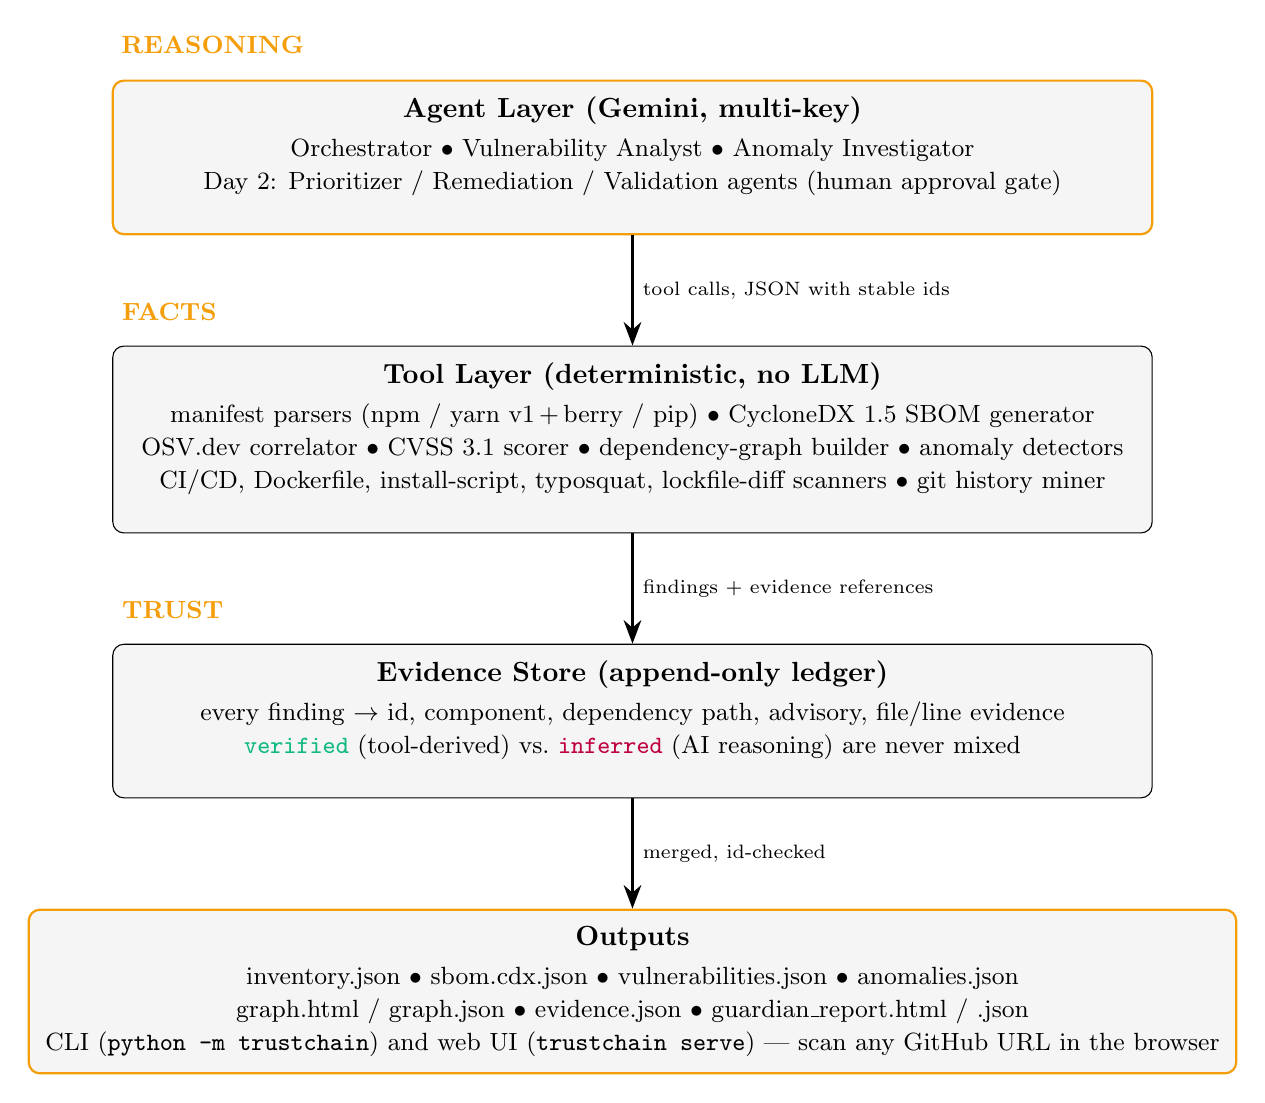
\begin{tikzpicture}[
  node distance=9mm,
  box/.style={draw, rounded corners, fill=gray!8, minimum width=13.2cm, align=center, inner sep=6pt},
  layer/.style={font=\bfseries\small, text=guardian},
  arr/.style={-{Stealth[length=3mm]}, thick}
]
\node[box, draw=guardian, thick] (agent) {
  \textbf{Agent Layer (Gemini, multi-key)}\\[2pt]
  \small Orchestrator $\bullet$ Vulnerability Analyst $\bullet$ Anomaly Investigator\\
  \small Day 2: Prioritizer / Remediation / Validation agents
  \small (human approval gate)\\[-2pt]};
\node[layer, above=2mm of agent.north west, anchor=south west] {REASONING};

\node[box, below=14mm of agent] (tools) {
  \textbf{Tool Layer (deterministic, no LLM)}\\[2pt]
  \small manifest parsers (npm / yarn v1\,+\,berry / pip) $\bullet$ CycloneDX 1.5 SBOM
  generator\\
  \small OSV.dev correlator $\bullet$ CVSS 3.1 scorer $\bullet$ dependency-graph
  builder $\bullet$ anomaly detectors\\
  \small CI/CD, Dockerfile, install-script, typosquat, lockfile-diff scanners
  \small $\bullet$ git history miner\\[-2pt]};
\node[layer, above=2mm of tools.north west, anchor=south west] {FACTS};

\node[box, below=14mm of tools] (evidence) {
  \textbf{Evidence Store (append-only ledger)}\\[2pt]
  \small every finding $\rightarrow$ id, component, dependency path, advisory, file/line
  evidence\\
  \small \textcolor{codegreen}{\texttt{verified}} (tool-derived) vs.\
  \textcolor{purple}{\texttt{inferred}} (AI reasoning) are never mixed\\[-2pt]};
\node[layer, above=2mm of evidence.north west, anchor=south west] {TRUST};

\node[box, below=14mm of evidence, draw=guardian, thick] (out) {
  \textbf{Outputs}\\[2pt]
  \small inventory.json $\bullet$ sbom.cdx.json $\bullet$ vulnerabilities.json $\bullet$
  anomalies.json\\
  \small graph.html / graph.json $\bullet$ evidence.json $\bullet$ guardian\_report.html
  / .json\\
  \small CLI (\texttt{python -m trustchain}) and web UI (\texttt{trustchain serve})
  \small --- scan any GitHub URL in the browser
};
\draw[arr] (agent) -- node[right, font=\scriptsize] {tool calls, JSON with stable ids} (tools);
\draw[arr] (tools) -- node[right, font=\scriptsize] {findings + evidence references} (evidence);
\draw[arr] (evidence) -- node[right, font=\scriptsize] {merged, id-checked} (out);
\end{tikzpicture}
\caption{TrustChain-AI architecture. Agents cannot create, delete, or alter findings;
they can only annotate entries that already exist in the evidence ledger.}
\label{fig:architecture}
\end{figure}

\subsection{Why agents cannot hallucinate findings}

Three mechanisms make the reasoning layer safe by construction:

\begin{enumerate}[itemsep=2pt]
  \item \textbf{Stable identifiers.} Every finding entering the agent layer carries an
        id (T-0001, T-0002, \dots) from the evidence ledger.
  \item \textbf{Contract prompts.} Each agent's system prompt requires a single JSON
        object \texttt{\{"analyses": \{"<id>": \{...\}\}\}} using only given ids.
  \item \textbf{Id-filtered merge.} The orchestrator discards every key that does not
        exist in the input set before writing anything to a report. Malformed or
        truncated model output is dropped entirely---the tool-verified facts always
        survive.
\end{enumerate}

%=====================================================================
\section{Day 1 Pipeline}
%=====================================================================

\subsection{Step 1 --- Discover the supply chain}

Manifest and lockfile parsers walk the target repository (gitignored build folders
skipped) and build a component inventory:

\begin{itemize}[itemsep=2pt]
  \item \texttt{package.json} / \texttt{package-lock.json} (npm lockfile v2/v3, full
        \texttt{node\_modules} tree path resolution)
  \item \texttt{yarn.lock} (classic v1 \emph{and} Yarn Berry \texttt{\_\_metadata}
        format, including \texttt{@scoped/name@npm:range} resolution)
  \item \texttt{requirements.txt} (PEP~508-style specifier parsing)
\end{itemize}

Each component records ecosystem, name, version, scope (direct/transitive), origin,
dependency edges and reverse dependencies. On the Strapi repository this yields
\textbf{3002 components (412 direct, 2590 transitive)}.

\subsection{Step 2 --- Build the supply chain view}

\begin{itemize}[itemsep=2pt]
  \item A \textbf{CycloneDX 1.5 SBOM} is generated with package URLs
        (\texttt{pkg:npm/\%40scope/name@version}), licenses and hashes
        (\texttt{sbom.cdx.json}).
  \item A directed \textbf{dependency graph} (networkx) is built: ROOT $\rightarrow$
        direct components $\rightarrow$ transitive components, with 3003 nodes and
        7126 edges for Strapi. Interactive pyvis/vis.js renderings highlight vulnerable
        components in red; large graphs are reduced to the most-connected 250 nodes
        while always keeping every vulnerable node.
  \item \textbf{CI/CD and container inspection}: GitHub Actions workflows, Dockerfiles
        and package lifecycle scripts are scanned (Section~\ref{sec:anomalies}).
\end{itemize}

\begin{figure}[htbp]
\centering
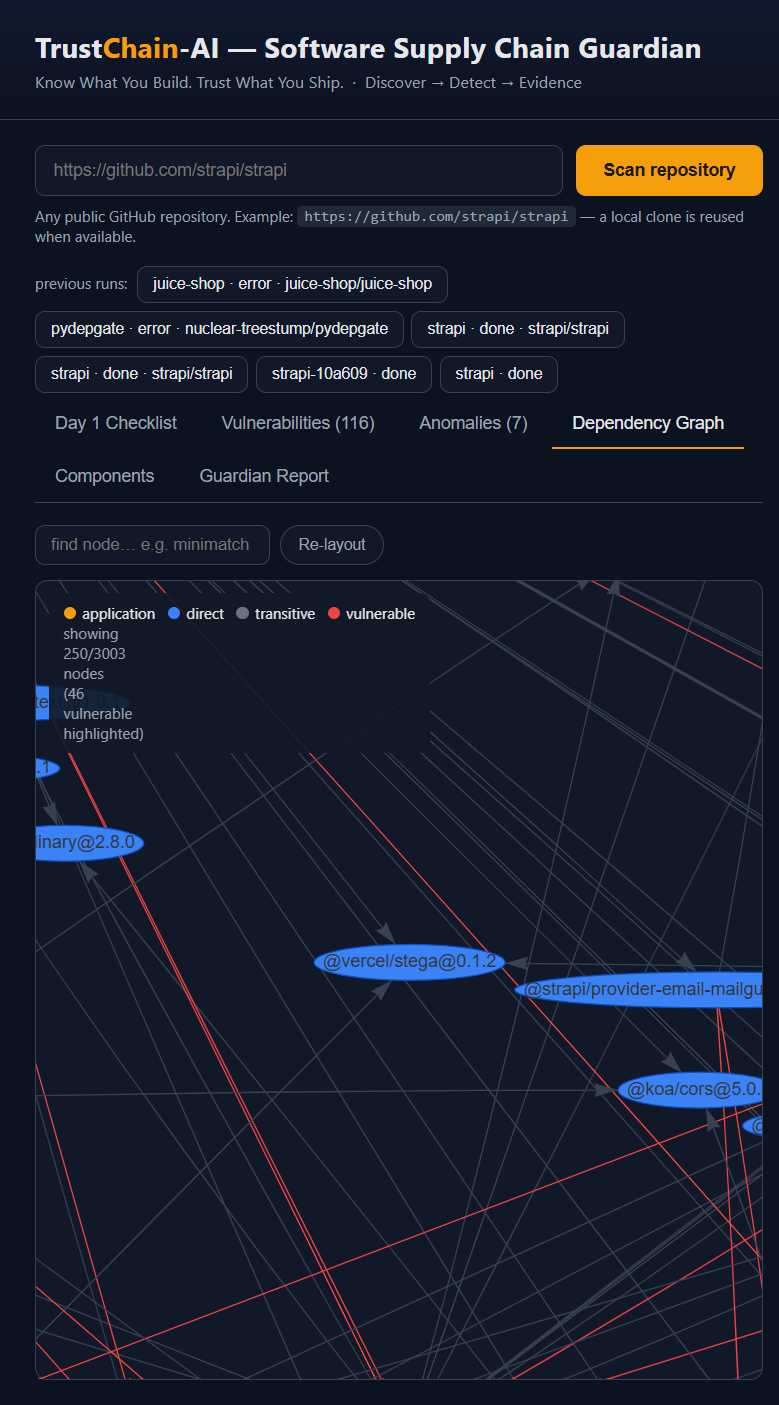
\includegraphics[width=\textwidth,height=0.82\textheight,keepaspectratio]{03-graph.png}
\caption{Interactive dependency graph in the web UI (Strapi: 3003 nodes reduced to the
250 most-connected, all 46 vulnerable components kept and highlighted in red).}
\label{fig:graph}
\end{figure}

\subsection{Step 3 --- Detect vulnerabilities}

Components are batch-queried against \textbf{OSV.dev} (500 per request, with a
disk cache shared across runs). For every advisory:

\begin{itemize}[itemsep=2pt]
  \item Severity is computed from the \textbf{CVSS~3.1 base-score vector} using the
        FIRST specification formula (no reliance on inconsistent upstream labels).
  \item Fixed versions are extracted from advisory ranges.
  \item The vulnerable component is \textbf{traced back to its root}: shortest
        dependency paths from every direct dependency are computed on the graph
        (e.g.\ \texttt{ROOT $\rightarrow$ @actions/http-client $\rightarrow$ undici
        $\rightarrow$ @fastify/busboy}).
\end{itemize}

The Strapi scan produces \textbf{116 findings}: 7 critical, 45 high, 38 medium,
13 moderate, 9 low, 4 unknown; 56 carry full dependency paths. Two findings are
\textbf{MAL- advisories} (malicious-package flags from OSV's malware database:
MAL-2026-1492, MAL-2026-1487) --- exactly the class of supply-chain attack that
CVE-only scanners miss.

\begin{figure}[htbp]
\centering
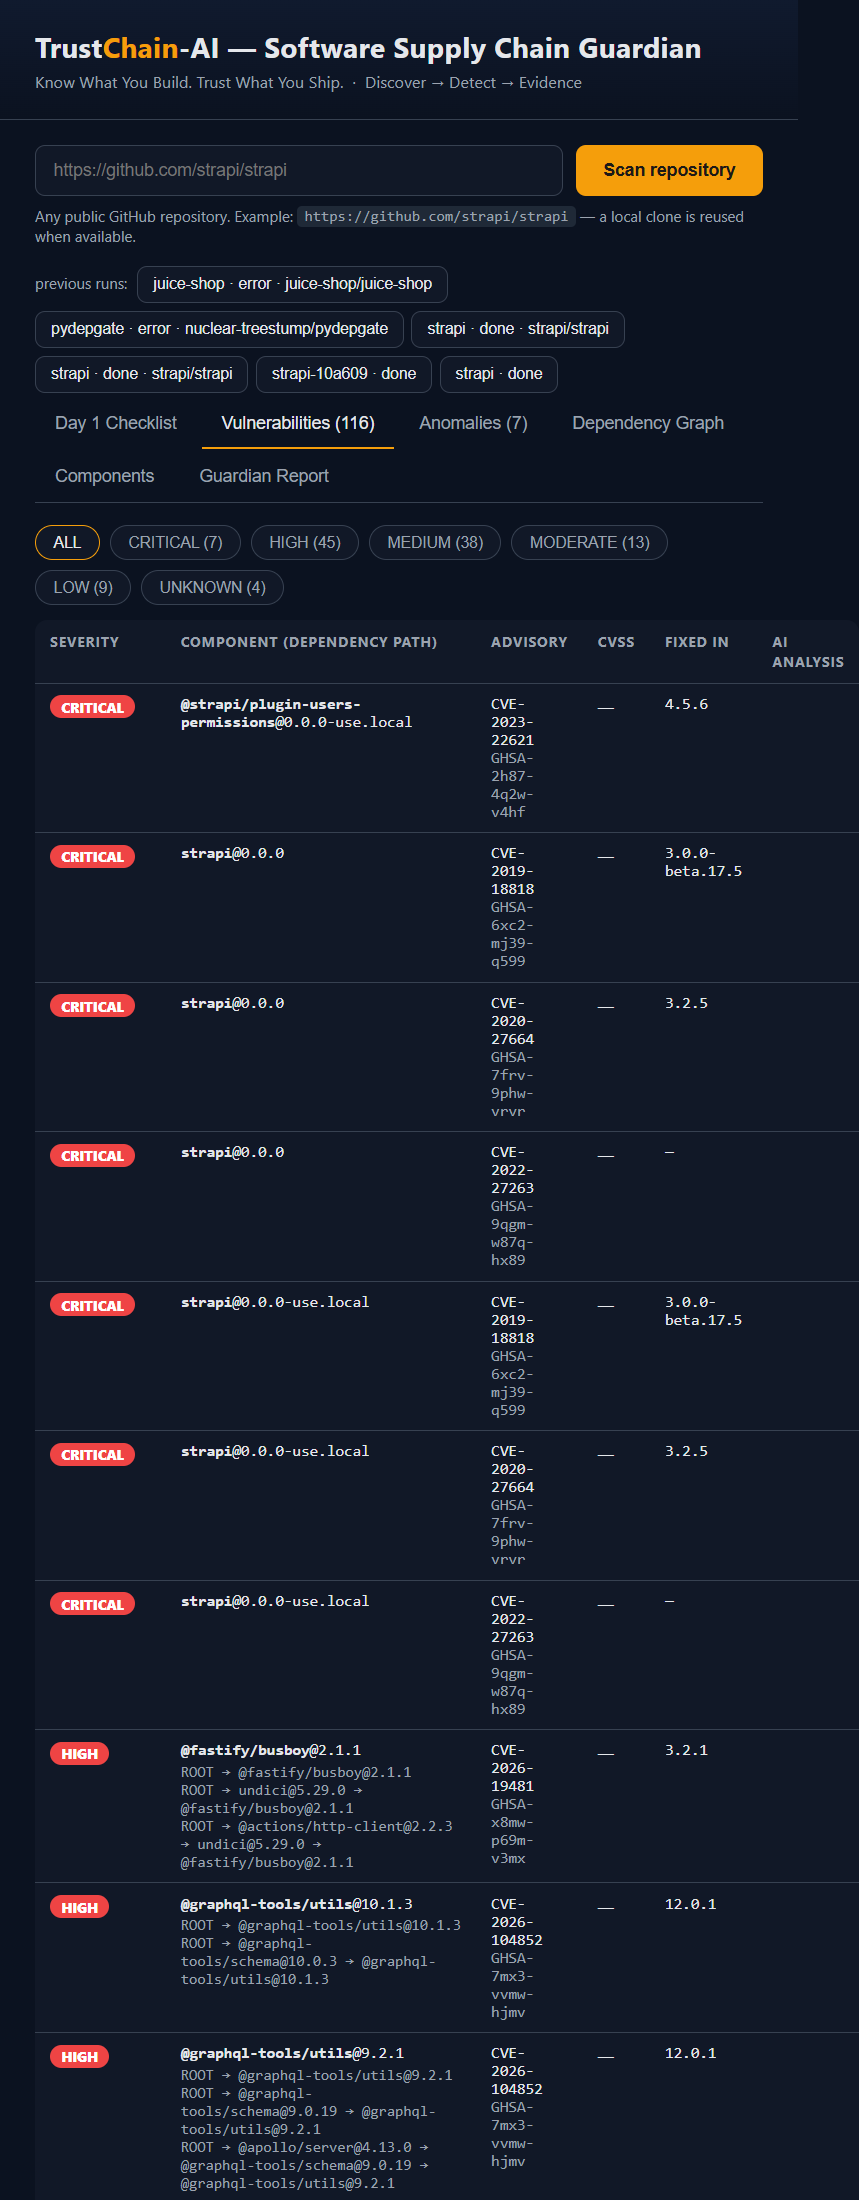
\includegraphics[width=\textwidth,height=0.82\textheight,keepaspectratio]{02-vulnerabilities.png}
\caption{Vulnerability browser: severity filter chips, dependency paths, CVSS scores
and fixed versions for all 116 findings.}
\label{fig:vulns}
\end{figure}

\subsection{Step 4 --- Detect suspicious changes}
\label{sec:anomalies}

Five deterministic detectors cover the hackathon's non-CVE anomaly list:

\begin{center}
\small
\begin{tabular}{@{}lll@{}}
\toprule
\textbf{Detector} & \textbf{Signals} & \textbf{Confidence} \\
\midrule
CI pinning        & \texttt{uses:} refs not SHA-40 pinned, \texttt{curl | sh}, & verified \\
                  & \texttt{pull\_request\_target} + checkout & \\
Container images  & \texttt{:latest} tags, unpinned digests & verified \\
Install scripts   & risky pre/post-install lifecycle scripts & verified \\
Typosquat         & Levenshtein distance $\le 2$ to popular package names & inferred \\
Lockfile diff     & per-package removed/added version sets between snapshots & verified \\
\bottomrule
\end{tabular}
\end{center}

The Strapi run flags \textbf{7 typosquat candidates}, each marked
\texttt{verified: false} with the matching distance stored as evidence --- an honest
``needs-review'' signal rather than a false certainty.

\begin{figure}[htbp]
\centering
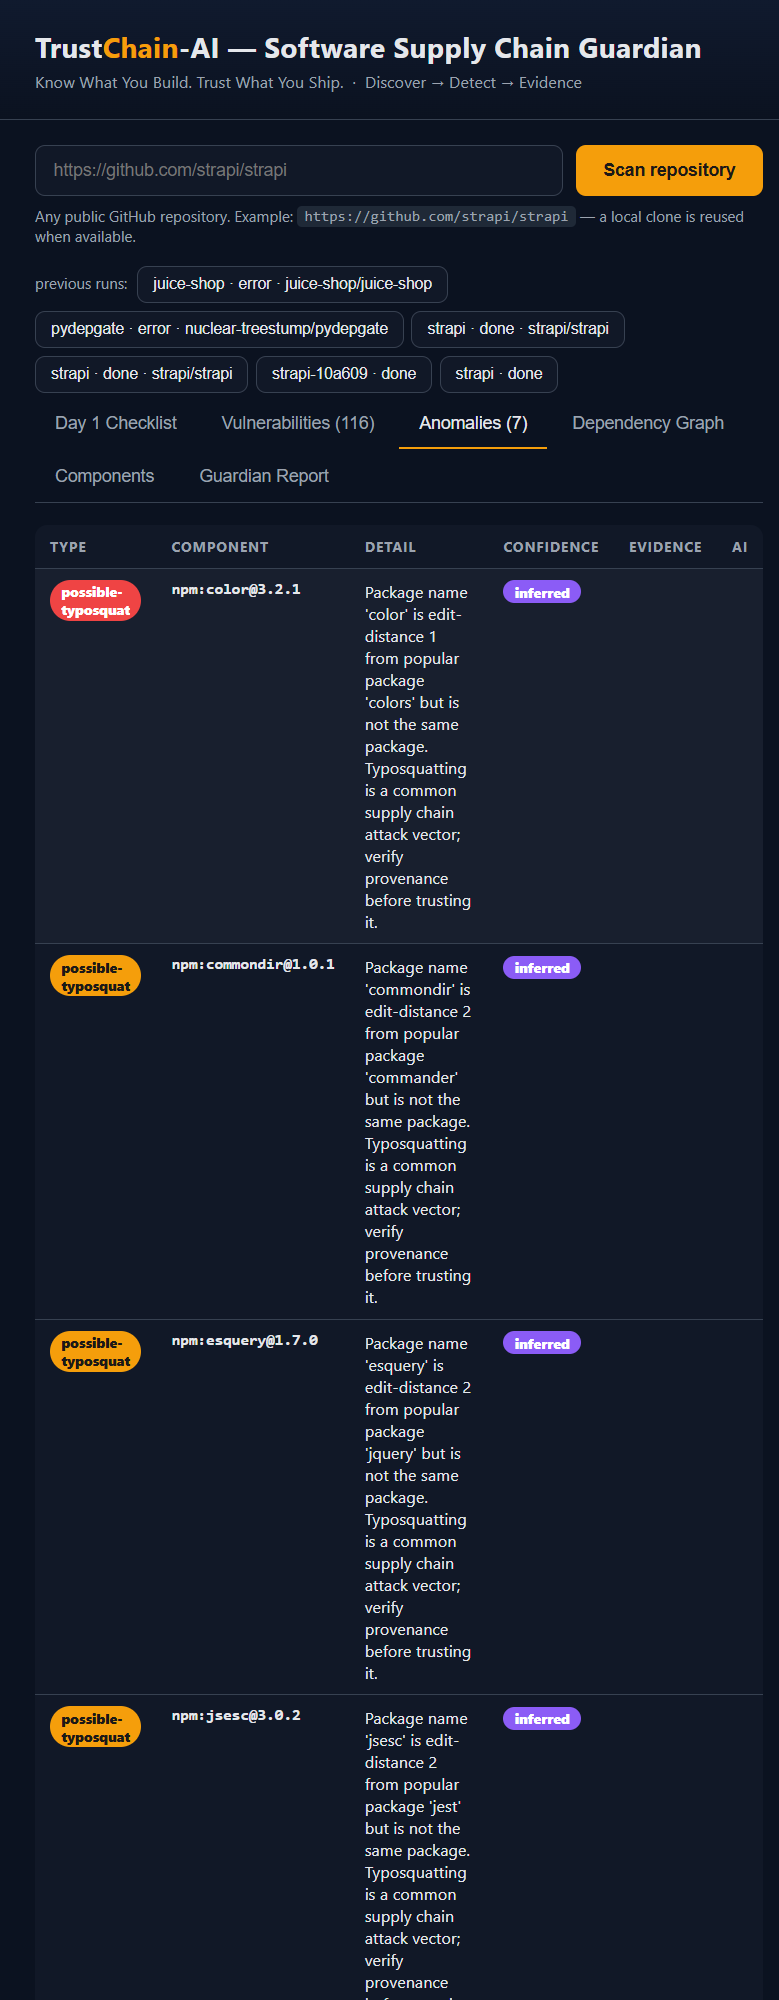
\includegraphics[width=\textwidth,height=0.82\textheight,keepaspectratio]{04-anomalies.png}
\caption{Anomaly table in the web UI: 7 typosquat candidates with Levenshtein-distance
evidence, each labelled \emph{inferred} pending human review.}
\label{fig:anomalies}
\end{figure}

\subsection{Step 5 --- Present evidence}

All findings enter the append-only \textbf{EvidenceStore} (123 entries on Strapi:
116 verified, 7 inferred). Each entry links its component, dependency path, advisory
id, fixed versions and file/line evidence. The final \textbf{Guardian Report}
(HTML + JSON) shows statistics, top-risk cards with paths and fixes, AI analysis blocks
explicitly labelled \emph{``inference, not verified evidence''}, and the full
methodology.

\begin{figure}[htbp]
\centering
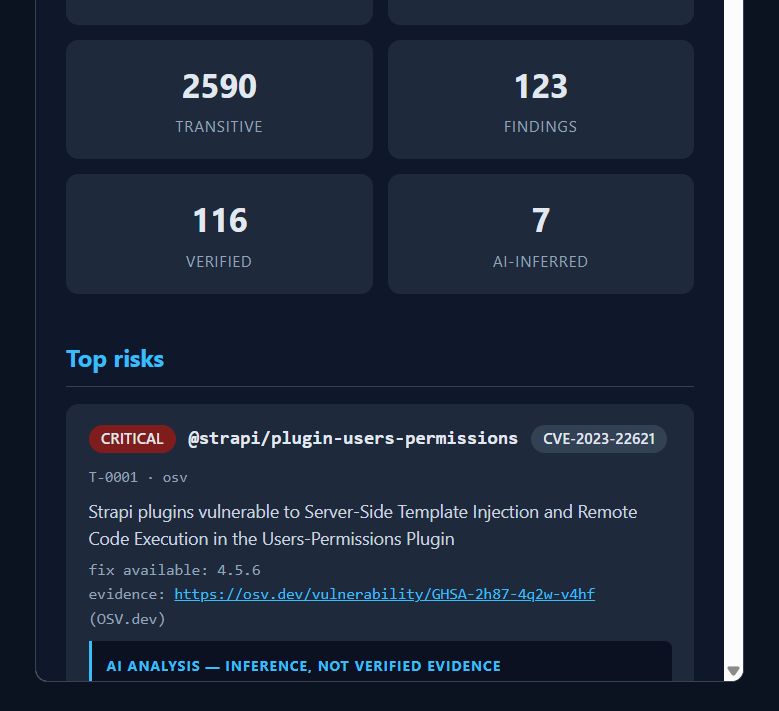
\includegraphics[width=0.85\textwidth,height=0.82\textheight,keepaspectratio]{05-report.png}
\caption{Guardian Report rendered inline in the web UI. The banner ``AI analysis ---
inference, not verified evidence'' separates agent reasoning from tool-verified facts.}
\label{fig:report}
\end{figure}

%=====================================================================
\section{Agent Layer in Detail}
%=====================================================================

\subsection{Gemini multi-key client}

The LLM layer uses Google's Gemini REST API (no vendor SDK) with a
\textbf{key pool and rotation} designed for the free-tier rate limits the team faced:

\begin{itemize}[itemsep=2pt]
  \item Up to \textbf{6 keys} are loaded from a git-ignored \texttt{.env} file
        (\texttt{GEMINI\_API\_KEY\_1..6}); only a placeholder template is committed.
  \item On \textbf{HTTP 429} (rate limit), \textbf{503} (model overloaded) or network
        timeouts, the client rotates to the next key and retries.
  \item If one model is globally unavailable (404/503 across all keys), it
        \textbf{falls back across models}: \texttt{gemini-3.8-flash}
        $\rightarrow$ \texttt{gemini-3.5-flash} $\rightarrow$ \texttt{gemini-2.5-flash}.
  \item If every key and model fails, callers degrade \emph{gracefully} to a
        tools-only report; a scan never fails because the LLM is unavailable.
\end{itemize}

\subsection{Agents}

\begin{center}
\small
\begin{tabular}{@{}p{3.4cm}p{4.2cm}p{5.6cm}@{}}
\toprule
\textbf{Agent} & \textbf{Input} & \textbf{Output per finding id} \\
\midrule
Vulnerability Analyst & verified CVE findings with paths & risk level, attention reason,
reachability note, confidence \\[3pt]
Anomaly Investigator & detector output with evidence & verdict (suspicious /
likely-benign / needs-review), reasoning, recommended action, confidence \\[3pt]
Orchestrator (deterministic) & scan artifacts + agent output & evidence ledger, merged
report, id-filtering and hallucination control \\
\bottomrule
\end{tabular}
\end{center}

Prompts embed the reasoning rules (many paths $\Rightarrow$ higher exposure;
\texttt{0.0.0-use.local} $\Rightarrow$ workspace package, not a registry bump;
distance-1 typosquats deserve scrutiny, distance-2 usually does not) and hard
constraints: only given ids, no invented CVEs, under 60 words, uncertainty marked with
lower confidence.

\textbf{Batching:} the analyst processes findings in \textbf{batches of 25} so model
responses never truncate; each batch is independently validated and merged. A malformed
batch is discarded, never retried into the report.

\subsection{Human approval gate}

Agents are physically incapable of merging, deploying or releasing anything. The
architecture has no code path that writes to the scanned repository; remediation
(Day~2 scope) requires a human to approve a proposed change before it is applied on a
branch. This satisfies the hackathon's responsible-AI requirement by construction, not
by policy.

%=====================================================================
\section{Retrospective Validation}
\label{sec:validation}
%=====================================================================

``How do you know the agent isn't making things up?'' The answer is a measurable,
reproducible harness that uses Strapi's own \emph{dependabot CVE-fix history} as
ground truth:

\begin{enumerate}[itemsep=2pt]
  \item \textbf{Mine} \texttt{chore(deps): bump X from A to B} commits from git history
        (12 commits analyzed).
  \item \textbf{Establish ground truth:} OSV is asked whether version A is affected and
        B fixed. Advisories that disappear across the bump mark a \emph{confirmed
        security fix} (6 of 12).
  \item \textbf{Rewind} to the pre-fix snapshot using a reusable \texttt{git worktree}.
  \item \textbf{Run the Guardian} on that snapshot, blind to the future fix.
  \item \textbf{Score} whether it flagged the known-vulnerable component and advisory,
        and whether the dependency-diff detector caught the version change.
\end{enumerate}

\begin{center}
\begin{tabular}{@{}lcc@{}}
\toprule
\textbf{Capability} & \textbf{Result} & \textbf{Recall} \\
\midrule
Vulnerability detection on pre-fix snapshots & 6/6 & \textbf{1.00} \\
Dependency version-change detection          & 11/12 & \textbf{0.917} \\
\bottomrule
\end{tabular}
\end{center}

The single miss is a multi-version lockfile where the removed/added version-set pairing
is ambiguous; the security advisory itself was still detected.

%=====================================================================
\section{Web Application}
%=====================================================================

The full pipeline is exposed as a web application (\texttt{python -m trustchain serve},
Flask + waitress in production):

\begin{itemize}[itemsep=2pt]
  \item \textbf{Scan by URL:} paste any public GitHub URL; the repository is shallow-
        cloned (local clones and a shared OSV cache are reused when available).
  \item \textbf{Live progress:} the 7-step pipeline (clone, discover, SBOM, OSV,
        anomalies, graph, report) runs in a background thread; the UI polls and fills
        the \textbf{Day~1 checklist} in real time with per-step details and evidence
        artifacts.
  \item \textbf{Findings browser:} vulnerability table with severity filter chips,
        dependency paths, CVSS scores, fixed versions and AI-analysis blocks;
        anomaly table with verified/inferred badges.
  \item \textbf{Interactive dependency graph} (vis.js) with vulnerable components
        highlighted, node search and re-layout.
  \item \textbf{Components explorer} (server-side search) and the full
        \textbf{Guardian Report} rendered inline.
  \item Only \texttt{github.com} URLs are accepted; path traversal in artifact
        endpoints is rejected; keys are never exposed to the browser.
\end{itemize}

\begin{figure}[htbp]
\centering
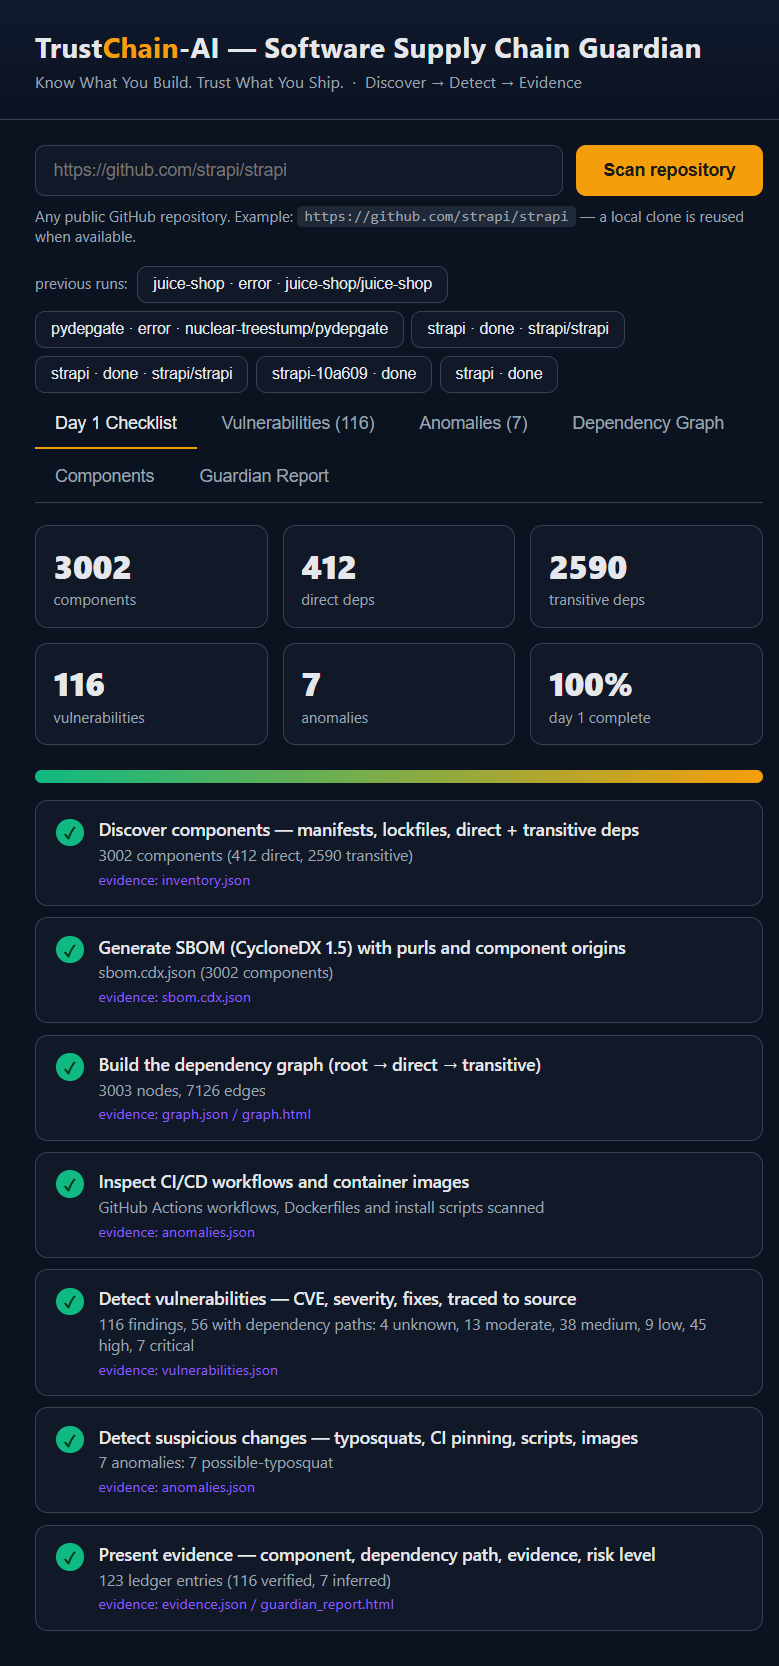
\includegraphics[width=\textwidth,height=0.82\textheight,keepaspectratio]{01-checklist.png}
\caption{Web UI after a completed Strapi scan: live statistics and the 7-step
Day~1 checklist at 100\%, with per-step evidence artifacts.}
\label{fig:checklist}
\end{figure}

\subsection{Deployment}

A Render blueprint (\texttt{render.yaml}) deploys the service on the free tier with
\texttt{waitress-serve}, a \texttt{/api/health} health check, and the Gemini keys
entered as secret environment variables in the dashboard.

%=====================================================================
\section{Responsible AI and Security}
%=====================================================================

\begin{itemize}[itemsep=2pt]
  \item \textbf{Facts before reasoning:} component lists, CVE matches, and diffs are
        produced by deterministic tools, never by the LLM.
  \item \textbf{Labelled uncertainty:} findings separate \texttt{verified} evidence
        from \texttt{inferred} reasoning with confidence levels; the report marks AI
        blocks as ``inference, not verified evidence''.
  \item \textbf{Hallucination control:} id-filtered merging discards anything the model
        invents; malformed output is dropped, not guessed at.
  \item \textbf{Human approval:} no auto-merge, deploy or release exists anywhere in
        the code base.
  \item \textbf{Sandbox scope:} all scanning is local, against cloned public
        repositories; no production systems, no publishing, no shared infrastructure.
  \item \textbf{Secret hygiene:} API keys live only in a git-ignored \texttt{.env} or
        platform environment variables; the repository contains a placeholder template
        only.
\end{itemize}

%=====================================================================
\section{Engineering Quality}
%=====================================================================

\begin{itemize}[itemsep=2pt]
  \item \textbf{41 automated tests} (discovery parsers, SBOM/graph, CVSS scoring,
        anomaly detectors, agent id-filtering, key rotation and model fallback,
        checklist computation, API endpoints) --- all passing.
  \item \textbf{Milestone-based history:} 11 commits from scaffold to deployment
        blueprint on \texttt{github.com/saiakhilesh5/TrustChain-AI}.
  \item \textbf{Graceful degradation everywhere:} no keys $\rightarrow$ tools-only
        report; overloaded model $\rightarrow$ key/model rotation $\rightarrow$
        tools-only; missing artifact $\rightarrow$ checklist marks the item pending
        instead of failing.
\end{itemize}

%=====================================================================
\section{Results Summary and Roadmap}
%=====================================================================

\begin{center}
\small
\begin{tabular}{@{}ll@{}}
\toprule
\textbf{Metric (Strapi)} & \textbf{Value} \\
\midrule
Components discovered      & 3002 (412 direct, 2590 transitive) \\
SBOM                       & CycloneDX 1.5, full purl set \\
Dependency graph           & 3003 nodes / 7126 edges \\
Vulnerability findings     & 116 (7 critical, 45 high, \dots) incl.\ 2 MAL- advisories \\
Findings with dep.\ paths  & 56 \\
Anomalies                  & 7 typosquat candidates (labelled inferred) \\
Evidence ledger            & 123 entries (116 verified / 7 inferred) \\
Validation recall          & 1.00 (vulnerabilities), 0.917 (version changes) \\
Automated tests            & 41 passing \\
\bottomrule
\end{tabular}
\end{center}

\textbf{Day 2 roadmap (in progress):} reachability-weighted prioritization, remediation
recommendations with expected risk reduction and rollback, human-approved branch
application, build/test/rescan verification with before-after SBOM diff, and
policy-as-code gating. Stretch goals: provenance verification (Cosign/Sigstore/SLSA),
dependency-confusion detection and continuous monitoring.

\vspace{2em}
\begin{center}
\textit{Core capabilities demonstrate completeness. Stretch goals demonstrate innovation.}\\
\textbf{Know What You Build. Trust What You Ship.}
\end{center}

\end{document}
